\documentclass[11pt,letterpaper]{article}
\usepackage[margin=1in]{geometry}
\usepackage[utf8]{inputenc}
\usepackage[T1]{fontenc}
\usepackage{hyperref}
\renewcommand{\familydefault}{\sfdefault}
\usepackage{helvet}
\pagestyle{empty}
\usepackage[kerning=true]{microtype}
\usepackage{parskip}
\usepackage{sansmath}
\usepackage{graphicx}
\usepackage{sidecap}  
\sidecaptionvpos{figure}{c}
\usepackage{float}
\usepackage{color, soul}
% Feel free to use additional packages for glosses, figures, whatnot.
\usepackage[dvipsnames]{xcolor}
\newcommand{\mf}[1]{\textcolor{BurntOrange}{[MF: #1]}}
\newcommand{\pt}[1]{\textcolor{Cerulean}{[PT: #1]}}
\newcommand{\bvt}[1]{\textcolor{ForestGreen}{[BvT: #1]}}
% The next bit is for reserving sufficient space for authors,
% affiliations, and e-mail address.  No need to change for initial
% anonymous version.  For the final version, replace the
%\toggletrue{anonymous} %with \togglefalse{anonymous} to de-anonymize.
\usepackage{etoolbox}
\newtoggle{anonymous}
\toggletrue{anonymous}

\renewcommand{\title}[1]{\textbf{#1}\\}
\newcommand{\authors}[1]{\iftoggle{anonymous}{\phantom{#1}}{#1}\\}
\newcommand{\email}[1]{\iftoggle{anonymous}{\phantom{#1}}{#1}}

\begin{document}

% First page:

% Insert title, authors, affiliations, and e-mail address in the next three lines:

\title{The role of relevance, competence and priors for scalar implicatures}
\authors{Michael Franke (University of T\"ubingen), Bob van Tiel (Radboud University), Polina Tsvilodub (Osnabr\"uck university)}
\email{pstvilodub@uos.de}

% Here goes the main text of your abstract:

If someone says "Anna ate some cookies." the hearer of this sentence might infer the upper-bounded reading that Anna ate \textit{some, but not all} cookies. Similarly, given the sentence "Donald ate a donut or a pretzel." one might infer an exclusive interpretation, i.e., that Donald ate either \textit{the donut or the pretzel, but not both}. 
Both of these inferences are usually explained as a variety of \textit{scalar implicature (SI)}. SIs rely on lexical scales consisting of words that are ordered in terms of informativeness, like $\langle$some, all$\rangle$ and $\langle$or, and$\rangle$. If a speaker uses an informationally weaker term (e.g., ``some''), they may imply that the corresponding stronger alternative (e.g., ``all'') is false [2,3]. %: if the stronger alternative was true, a rational agent would have used the stronger utterance; but since she did not, she must have lacked the evidence for using ``all'' 
%(Grice, 1975).
%Some prior work addresses the influence of sentence structure, or of specific linguistic markers on the robustness of SIs (Li, 2021). Moreover, 
Crucially, prior research suggests that the robustness of SIs varies across contexts [6].
Here, we investigate the effects of three factors that have been argued to influence the robustness of SIs: (1) \textit{relevance} of the stronger alternative to the listener, (2) the \textit{competence} of the speaker about the truth of the stronger alternative, and (3) the \textit{prior probability} that the stronger alternative is true [1,3,5]. However, their influence was mostly investigated in isolation in prior work. We explore how these three factors interactively influence the robustness of SIs associated with the triggers ``some'' and ``or''. Simultanously, we directly compare whether the two triggers are both influenced by these factors.

In our web-based rating study, participants read background stories which were designed to vary in terms of the strength of the three factors of interest (prior probability $\times$ competence $\times$ relevance, for each trigger), manipulated within-subjects. 
On critical trials, participants were asked to rate three sentences on a scale ranging from ``certainly true'' to ``certainly false'' (converted to 0--100), one per factor. The background story ended with
one of the characters in the story making an utterance containing ``some'' or ``or''. Participants then
had to indicate the probability of an SI-enriched paraphrase of that utterance. We thus obtained
judgements on the contextual factors, and on the robustness of the SI (s. \url{https://tinyurl.com/3ru9sdja} for transcripts). Based on
the literature, we expected higher likelihood ratings for the SI-enriched paraphrase if the
alternative was perceived as highly relevant, the speaker was judged as highly competent, and
the stronger alternative was viewed as a priori unlikely. Each participant saw eight stories (four per trigger)
sampled from 32 stories/trigger, randomly shuffled with eight structurally similar attention checks
and comprehension questions.

%(71  excluded following preregistered exclusion criteria).
We analysed data from 206 participants recruited through Prolific; their ratings were z-scored within each factor by-participant. We analysed the results using a Bayesian linear mixed effects model, regressing the implicature likelihood rating against the fixed effects of all factor ratings by the same participant for that vignette, the effect of trigger, all interactions and maximal tractable random effects structure. Participants' factor ratings agreed well with the prior classification of the items (Fig.~\ref{by-item-ratings}, colors).
%Consistent with predictions of the SI account, for the trigger ``some'', we find a clear negative prior probabilty effect of the stronger alternative ``all'' being true (probability of the effect of prior being smaller than 0.05: $P = 0.999$). 
As predicted, participants were more likely to derive the SIs of ``some'' and ``or'' when judging speaker competence as high ($P=0.999$ for ``some'',  $P=0.993$ for ``or'' for the effect being $<0.05$, Fig.\ref{posteriors} for all results). 
Participants were also more likely to derive the SI of ``some'' when judging the prior probability of ``all'' as low ($P =  1$ for effect $<0.05$), which was not the case for ``or''. %Interestingly, we did not observe a credible effect of prior probability in the case of ``or''.
Finally, we did not observe credible effects of relevance for either trigger.

%For the trigger ``or'', we only find a positive effect of competence ($P =  0.993$). 
Further, we computed exploratory pairwise correlations of all the predictors. While no correlations were found for ``some'', we find a significant correlation between the prior and the relevance effects for ``or'' ($R^2 = -0.106, p=...$), and a significant correlation between competence and relevance ($R^2 = 0.127, p=...$) for ``or''. This suggests that these factors might be interdependent in case of ``or''.

These results partly confirm the predictions. First, the effects of competence show that both types
of SIs rely on epistemic reasoning. However, only in the case of “some” did the robustness of
the SI vary with the prior likelihood that the alternative is true. Although we did not find such an
effect of prior probability for “or”, exploratory analyses indicate that this null effect may be due to a
correlation with the other two factors. Perhaps most forcefully, our results speak against the idea
that SIs are modulated by considerations of relevance. Our study thus provides insight into the
contextual features that enter into people’s decision as to whether or not derive an SI.
%Overall, our results support the SI account, but also indicate that these factors might have a more fine-grained influence on the robustness of SI generation in combination.%, especially for disjunction interpretation.
%Overall, the results provide moderate evidence for the scalar implicature account of ``some'' and ``or'', but also indicate that there might be intricate dependencies between the factors' influence on the robustness of SI, especially for disjunction interpretation.
\newpage

% Second page for additional materials, example stimuli, graphs, tables, references:


\begin{SCfigure}[1.7]
  % \makebox[\linewidth][c]{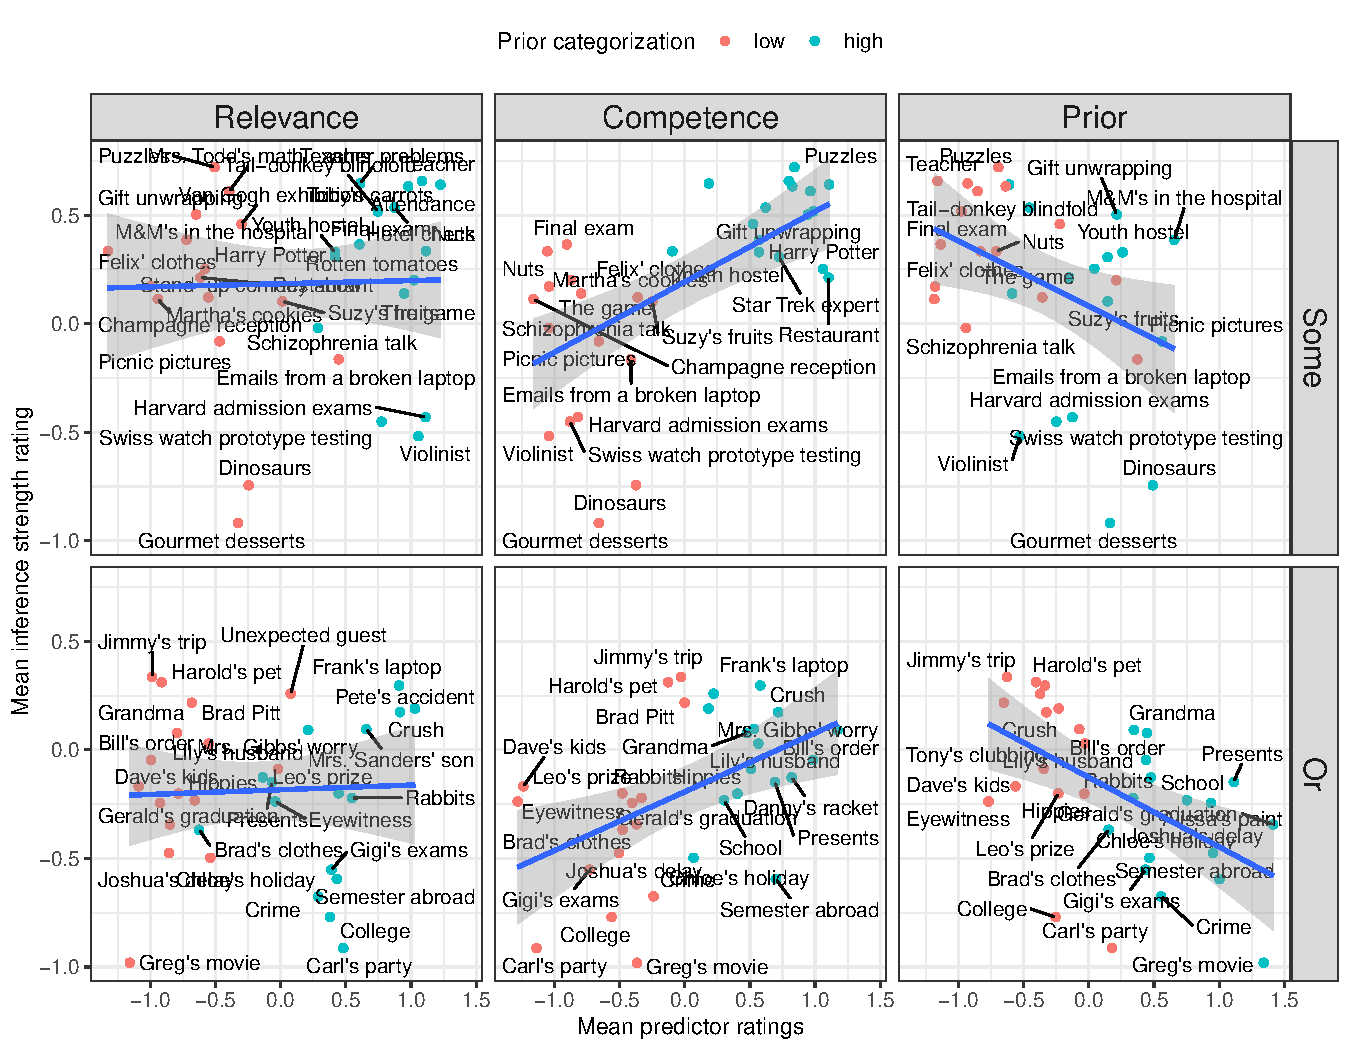
\includegraphics[width=0.7\linewidth]{byItem-ratings.pdf}}%
  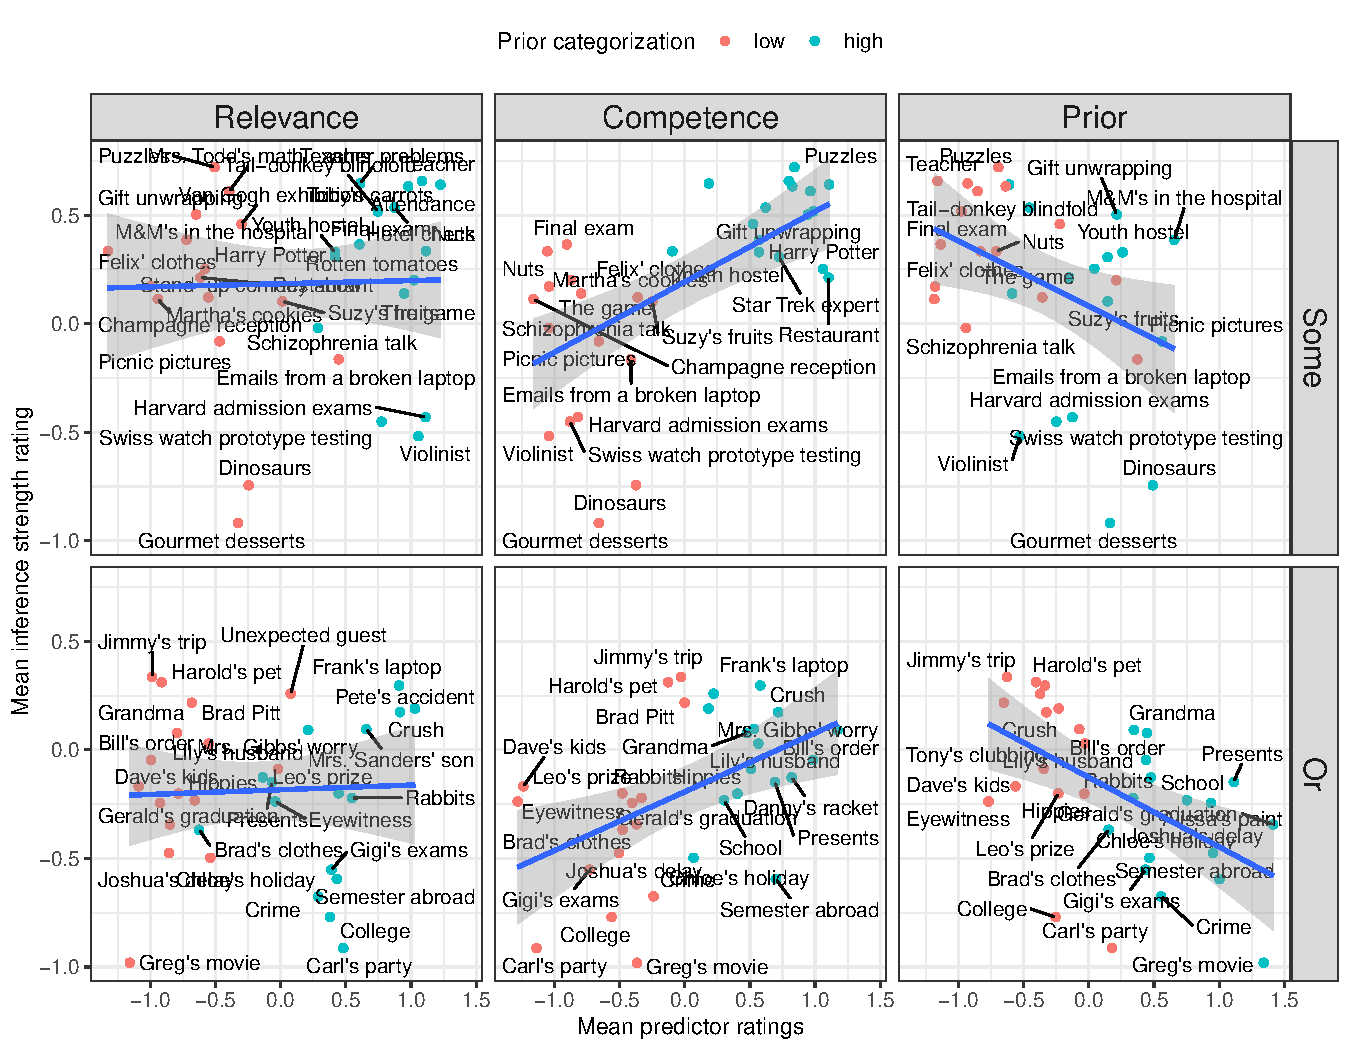
\includegraphics[scale=0.5]{byItem-ratings.pdf}
 \caption{Relating ratings for relevance, competence and prior statements (x-axis) to
ratings for the strength of pragmatic enrichments (y-axis). The top row shows ratings,
averaged for each story for ``some'' (enriched to ``some, but not all''). The bottom row shows ratings, averaged for each story for ``or'' (enriched to ``A or B, but not both'').}
    \label{by-item-ratings}
\end{SCfigure}

\begin{figure}   
    \makebox[\linewidth][c]{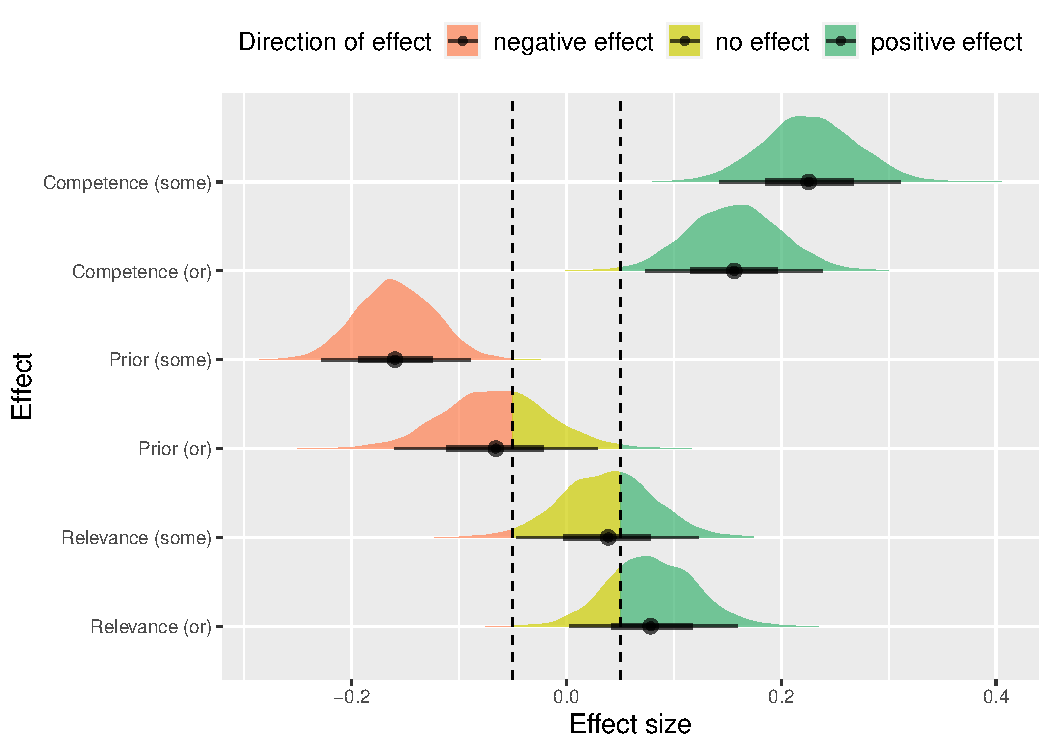
\includegraphics[scale=0.7]{posterior-effects.pdf}}
    \caption{Distributions of posterior samples for the effects of each predictor for each trigger (y-axis). The colors indicate the fraction of the distribution density corresponding to a positive, no or a negative effect. \newline \textbf{References:} [1] Degen, J., Tessler, M. H., \& Goodman, N. D., In \textit{Proceedings of CogSci}, 2015 [2] Geurts, B., \textit{Quantity Implicatures}, 2010 [3] Goodman, N. D., \& Stuhlm\"uller, A., In \textit{Topics in Cognitive Science}, 5(1), 2013 [4] Grice, H. P. In \textit{Syntax and semantics, vol. 3: Speech acts}, 1975 [3] Horn, L. R., \textit{On the semantic properties of logical operators in English}, 1972 [5] Sperber, D., \& Wilson, D., \textit{Relevance: communication and cognition}, 1995  
    }
    \label{posteriors}
\end{figure}

%\begin{SCfigure}[1.7]
%    \includegraphics[ scale=0.5]{amlap_expt4_double_mod2.pdf}
 %   \caption{Pilot Results: Inferred basic-level comparison classes (e.g. ‘...big relative to other \textit{dogs}’) when the directly modified subordinate N (‘big Great Dane’) appears in different syntactic positions (x-axis).\newline
%    \newline \textbf{References:} [1] Kamp, J., In \textit{Formal semantics of natural language}, 1975  [2] Kennedy, C., \textit{Linguistics and Philosophy, 30(1)}, 2007 [3] Tessler, M. H.; Lopez-Brau, M.; Goodman N. D., In \textit{39th annual meeting of the Cognitive Science society}, 2017
%    \label{double-mod}[4] Reboul, A., In \textit{Language typology and language universals, an international handbook, vol.1}, 2001}
%\end{SCfigure}

\newpage

% Optional third page for additional information if the investigated language is not English:
\end{document}
